%! Author = giaco
%! Date = 16/05/2024

\chapter{Method}
\label{ch:method}
As already highlighted in Ch.~\ref{ch:introduction} and Ch.~\ref{ch:related_work}
a typical RL setting consists of an agent that receives as input the state of the environment and has to learn a policy to solve a specific task.
Most of the training time is spent trying to get a useful representation of the state, which is then used to learn the policy.
The focus of this work is to simplify as much as possible the representation learning of current RL algorithms leveraging prior knowledge and letting the agent focus on learning the actual policy to solve the task.
Many previous works already, mentioned in Sec. \ref{sec:fm_rl}, share the idea of leveraging FMs to enhance the state representation facilitating the transfer of world knowledge and simplifying the RL training process.
Almost none of them have tried to combine multiple models at the same time.
Our methodology is designed to use multiple models at the same time, instead of just one, to enhance the efficiency and effectiveness of RL agents by leveraging a set of pre-trained models tailored to the current task.

Our work poses two main questions, how to represent skills for an RL agent and how to combine them.
To answer the first question, FMs present themselves as good candidates, as they provide a general representation of the environment.
These representations can be leveraged in RL to speed up the learning process and improve performance on complex tasks.
Using FMs' knowledge, RL agents can achieve higher efficiency and effectiveness, even in environments with sparse rewards or limited data.
First, our work proposes a set of basic abilities like humans have.
RL agents are equipped with these FMs, which serve as the prior knowledge needed to generate diverse representations of the environment.
While agents interact with the environment, the current observation is collected and processed through each pre-trained model.
This process produces multiple perspectives or views of the world, each distinctively represented according to the particular model used.
%These features embody various aspects of the environment, providing the agent with a comprehensive and enhanced understanding of the current state.

As for the latter question, instead, this thesis aims to study how different FM embeddings can be combined in several ways to compute a rich and informative representation of the environment.
We focus on how to effectively combine their latent representations to improve agents' performance.
The challenge lies in integrating these possible divergent views into a single and enriched representation.
In order to achieve this, we employ a specialized combination module, that synthesizes the information from the various models into a single latent representation.
The intuition is that the enriched representation provides a comprehensive understanding of the current state of the environment, derived from the collective insights of the pre-trained models.
By using FMs, our approach significantly alleviates the RL agent's need to learn the environmental representation from scratch, allowing it to focus more on refining the action-mapping process.
This not only speeds up the learning process but also enhances overall performance by providing a well-structured and informative representation.

The architecture of our agents is divided into two main components, and it is shown in Fig.~\ref{fig:main}
The first part takes care of processing the current observation into multiple latent representations and then combines them into a single enriched representation.
We refer to this part as the \textit{Feature Extractor} module.
The second part is the \textit{Policy Learning} network, where the unified representation is fed into a small fully-connected neural network whose responsibility is to map the latent encoding to actions.


\begin{figure}[ht]
    \begin{center}
        %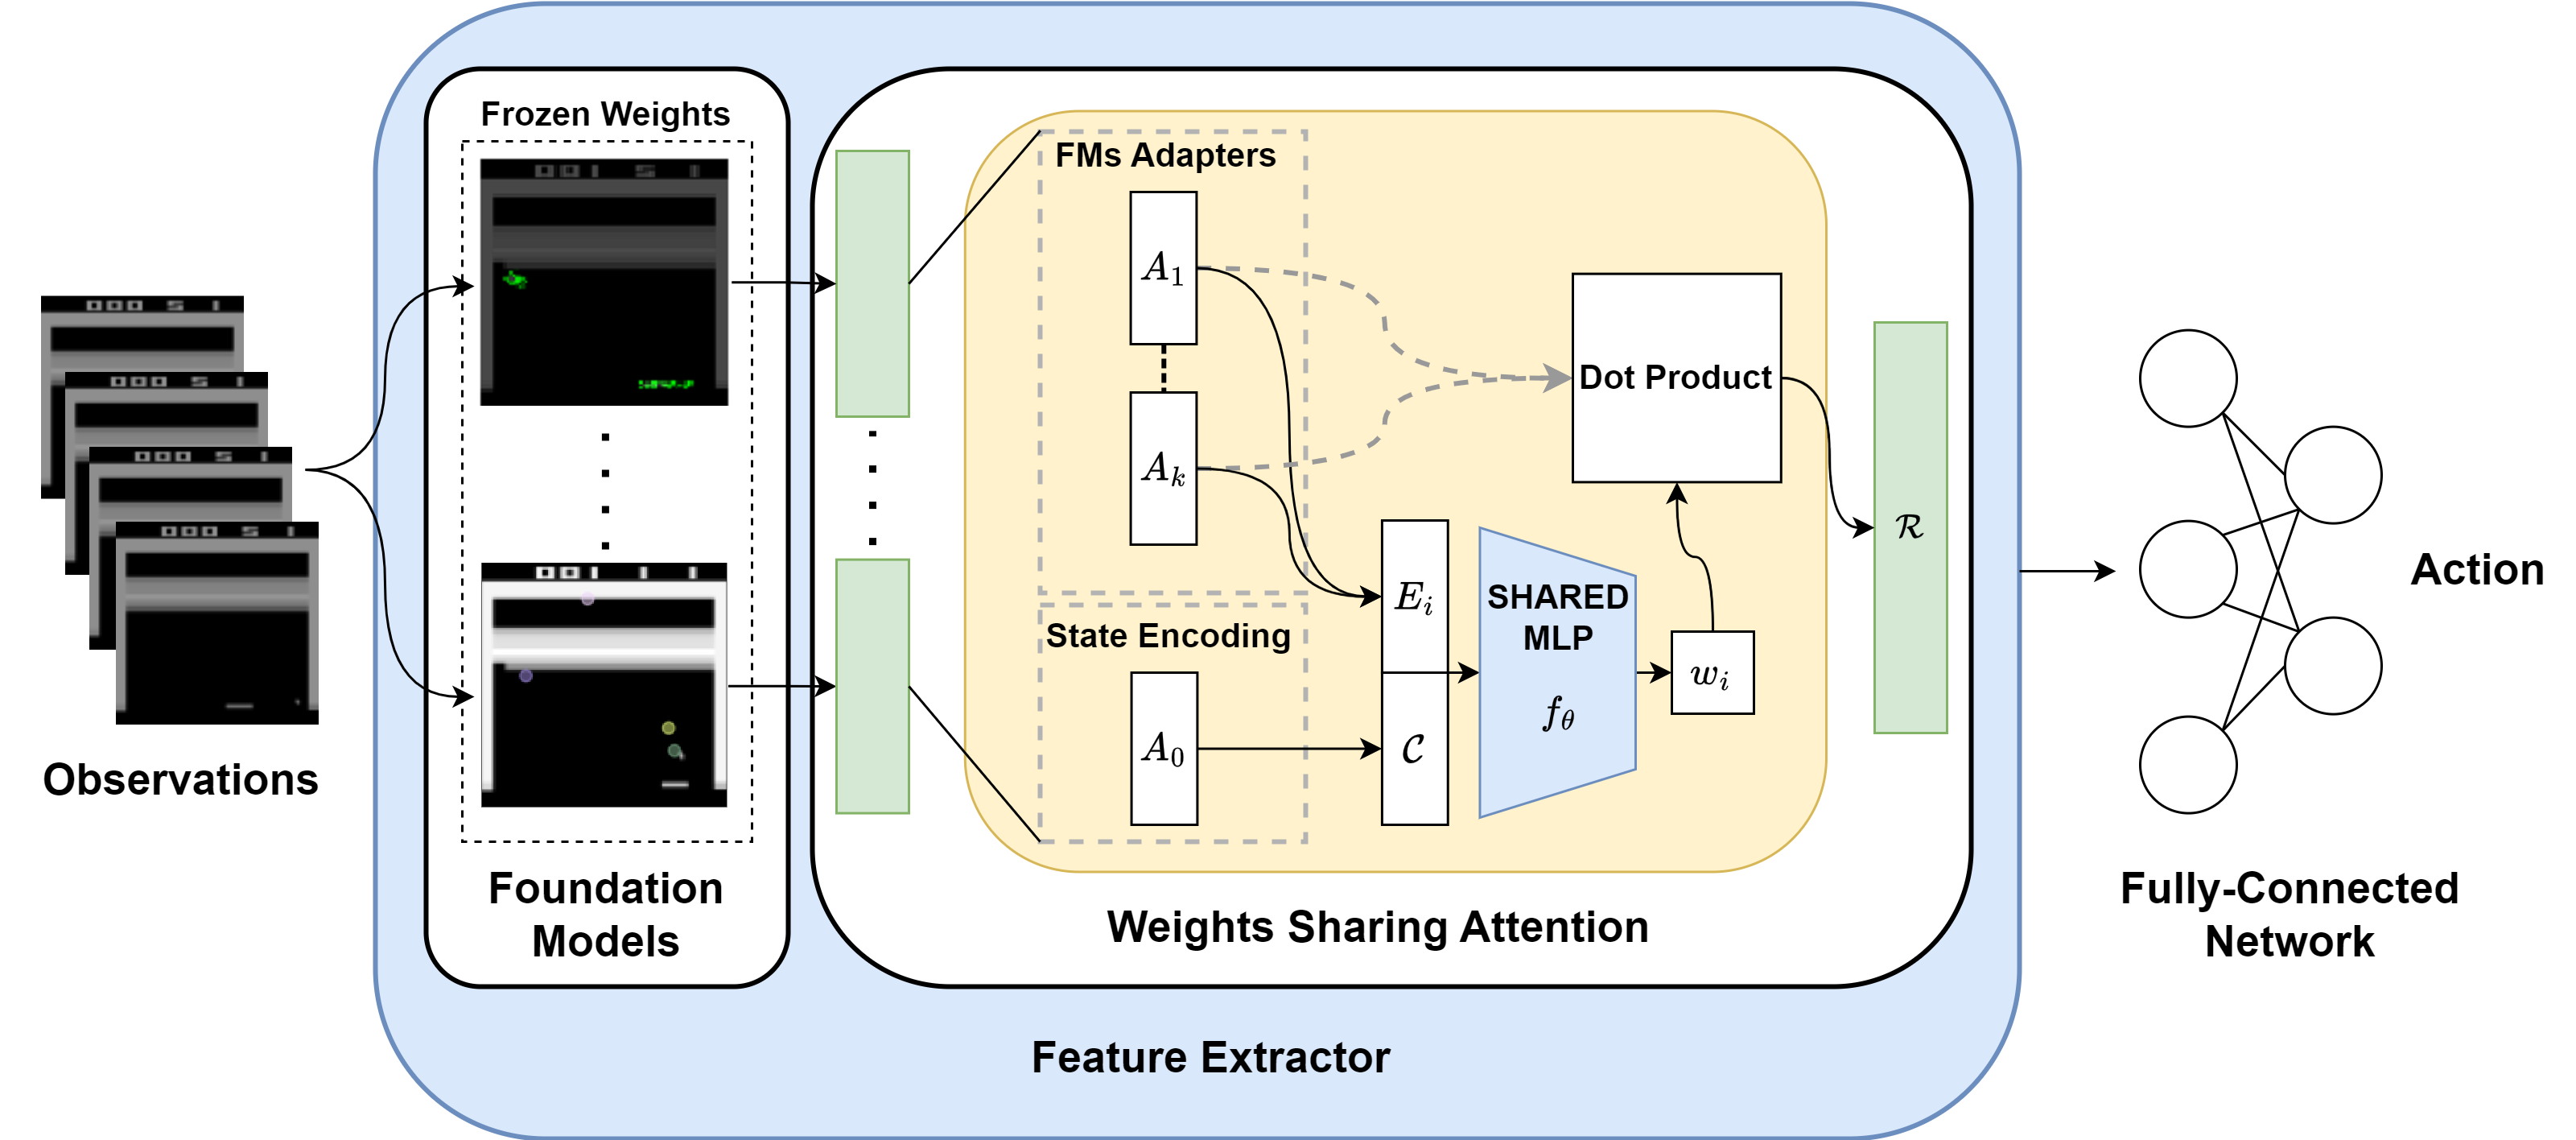
\includegraphics[width=1\textwidth]{images/main_architecture2}
        \fbox{\rule[-.5cm]{0cm}{4cm} \rule[-.5cm]{4cm}{0cm}}
    \end{center}
    \caption{General main architecture}
    \label{fig:main}
\end{figure}


In the following sections, we will describe in detail our methodology, and how we map information from observations to actions.
In particular, Sec.~\ref{sec:feature_extractor}, will describe how we designed the Feature Extractor module focusing on various combination techniques to merge the representations extracted by the FMs.
While Sec.~\ref{sec:policy_learning}, we will provide some information about the Policy Learning network.




% prova ad integrare se serve
%Besides our proposed methodology, we tested and compared the performance of several combination modules. All solutions act as interchangable modules inside the \texttt{Feature Extractor}, i.e. only need to replace the \textcolor{orange}{yellow} component in Figure \ref{fig:main_architecture}. Their output is a linear representation that is provided as input to the \texttt{Fully-Connected Network}. We report a rundown across all solutions:
%\begin{itemize}
%    \item \texttt{Linear} (LIN): pre-trained models' representations are linearized and concatenated.
%    \item \texttt{Fixed Linear} (FIX): embeddings are linearized to a predefined size, possibly using adapters to scale the information.
%    \item \texttt{Convolutional} (CNN): FMs' outputs are concatenated along the channel dimension. They are processed by a predefined number of convolutional layers and the resulting information is flattened to linear.
%    \item \texttt{Mixed} (MIX): this is a combination of the previous methods. Data coming from different spaces are dealt separately and then combined.
%    \item \texttt{Reservoir} (RES): inspired by \citet{gallicchio2017}, this approach leverages reservoir layers to combine models' representations.
%    \item \texttt{Dot Product Attention} (DPA): similarly to \texttt{Fixed Linear} the representations are reduced to a specific size - key and value. Via \texttt{scaled dot product attention} \citep{vaswani2017attention} we compute the final weighted representation using as query vector the representation obtained from the State Encoder.
%\end{itemize}




\section{Feature Extractor} \label{sec:feature_extractor}
The Feature Extractor module is the first part of our agent, it is responsible for processing the current observation and extracting a meaningful representation of the environment in a compact latent space.
It is composed itself of two main parts, the first part is a set of pre-trained models, while the second part of the module is the combination module, which is the core of the Feature Extractor.
%a sentence to refer the subsections

\subsection{Foundational Models}\label{subsec:foundational-models}
Agents receive as input the last four frames of the game, which are stacked together to form the observations.
Starting from the observations, the first step of our methodology is to gather information from the environment at different levels of abstraction.
We equipped our agents with a set of $k$ pre-trained models $\Psi = \{\psi_1, \psi_2, \ldots, \psi_k\}$, capable of represent the current observation $\mathcal{O}$ under different perspectives.
Meaning that the models are pre-trained on different tasks.
During the training of RL agents, their weights are frozen in order to preserve the knowledge acquired during the pre-training phase and speed up the learning process.
In particular, we will have a set of $k$ embeddings $E^{FM}$ in output from the FMs, $E^{FM}_i = \psi_i(\mathcal{O})$.
The models operate both in the spatial field, so they output an embedding consisting of a set of feature maps, and in the linear field, so they output a one-dimensional vector.
This is the initial step of our methodology.
We will talk more in detail about the FMs selected in Sec. \ref{sec:exp_setup}

\subsection{Combination Modules}\label{subsec:combination-modules}
Continuing with the Feature Extractor module, the next step is to combine the representations extracted by the FMs.
Combining different FMs encoding is a challenging task, as each model provides a different view of the environment.
The goal is to merge these perspectives into a single enriched representation that captures the most relevant information.
To achieve this, we developed several combination modules, each with its own strengths and weaknesses.
All solutions act as interchangeable components, and we tested and compared their performance.
All combination modules have in common a first \textit{preprocessing step}, consisting of a set of adapters $\mathcal{A}^{s}$, called \textit{Spatial Adapters}, which are used for embeddings $E^{FM}_i$ that operate in the spatial field.
This set of adapters is implemented as two convolutional layers followed by a ReLU activation function.
This is done to resize the latent representation of the FMs to a fixed size, ensuring compatibility among different models.
While the FMs that operate in the linear field are left as they are.

We will present one by one all the combination techniques that we have developed to merge the representations extracted by the FMs, with a particular emphasis on the Weight Sharing Attention module, which is the component that we propose as a solution to the problem of combining different FMs in an effective way, and we think that it deserves more relevance.
Their output is a linear representation that is provided as input to the \textit{Fully-Connected Network}.

\subsubsection{Weight Sharing Attention}\label{subsubsec:wsa}
With a view to lifelong learning agents, the aim is therefore to equip the agent with prior skills that can be changed or improved over time to adapt to new unseen tasks.
To this end, a model capable of re-adapting to new abilities with little or no effort is needed.
To facilitate the integration of different pre-trained models, we propose WSA\@.
The WSA module leverages the concept of \textbf{weight sharing}, as seen for the first time in CNNs~\citep{fukushima1980neocognitron}, and \textbf{attention}~\citep{vaswani2017attention} principles to efficiently merge outputs from diverse FMs.
In specific, WSA dynamically adjusts the weights assigned to each pre-trained model based on the current context, emphasizing the most relevant models for the current state.

This module, depicted in Fig. \ref{fig:wsa_main_architecture}, is designed in this way.
It receives as input the representation extracted by the FMs, on which it applies the preprocessing step described before.
Then, spatial embeddings are flattened to obtain a one-dimensional vector.
WSA module is equipped with another set of adapter, called \textit{Linear Adapters} $\mathcal{A^{l}}$, where each adapter $\mathcal{A^{l}_i}$ is a small neural network consisting of a single linear layer followed by a non-linearity layer, in this case, a ReLU activation function.
The adapter is used to learn a representation of the model's output and also to resize the linear latent representation of the FM to a fixed size.
This guarantee consistency between various models.
As a result of this operation, we obtain an embedding for each FM representation, called $E^{l}_i$, of a predefined size.


\begin{figure}[ht]
    \begin{center}
        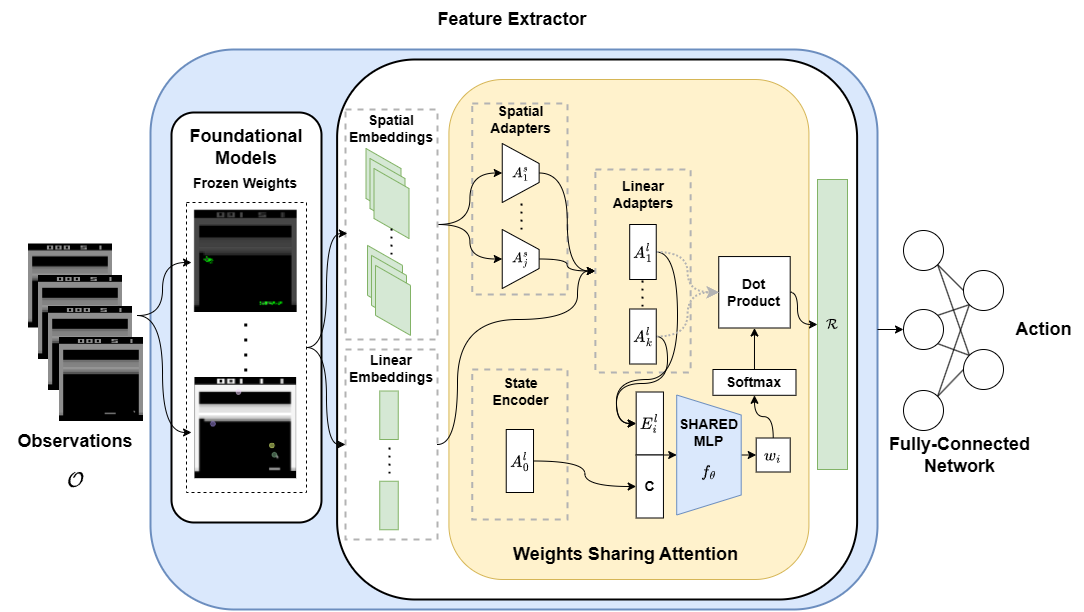
\includegraphics[width=1\textwidth]{images/wsa_main_architecture}
    \end{center}
    \caption{In Figure, we show all the information flow from observation to actions and the architecture of the WSA module. The last four frames are stacked together and passed as input to the FMs and their adapters $\mathcal{A}_1, \dots \mathcal{A}_k$ to obtain an embedding of the current state $E^l_i$. A State Encoder $\mathcal{E}$ and its adapter $\mathcal{A}^l_0$ compute an encoding of the state, that will be used as context $\mathcal{C}$. A shared MLP layer takes as input the context $\mathcal{C}$ and the representation of the $i^{th}$ FM, $E^l_i$, and produce the weight for that specific model. The final enriched representation $\mathcal{R}$ is obtained from the weighted summation between each weight $w_i$ and its respective embedding $E^l_i$. $\mathcal{R}$ is given as input to agents' \textit{Fully-Connected Network}.}
    \label{fig:wsa_main_architecture}
\end{figure}


Among the provided FMs, one is used as \textbf{State Encoder} $\mathcal{E}$ to compute a representation of the current state, which serves as \textit{context} $\mathcal{C}$ for the attention mechanism.
The State Encoder produces a spatial embedding of the current observation.
Here we do not use a spatial adapter to preprocess the output of the State Encoder, we just flatten the representation to obtain a linear embedding.
A linear adapter $\mathcal{A}^{l}_0$ of the same shape of the others is used to resize the latent representation to a fixed size, and this will be the context $\mathcal{C}$.

To compute the attention weights, we use a shared MLP $f_\theta$ that takes as input the context $\mathcal{C}$ concatenated with the single embedding $E^{l}_i$ of each FM\@.
This MLP outputs the model-specific weight $w_i$ to determine the contribution of each model in the final representation.
Weights are stacked together and passed through a softmax function to ensure that they sum to one.
It is important to note that this MLP is shared across all models, ensuring uniform weight computation.
By dynamically adjusting weights based on the current context, WSA emphasizes the most relevant models for any given situation, resulting in a more accurate and adaptable representation.
The final representation $\mathcal{R}$ is computed using the weights for all pre-trained models and computing a weighted sum of their embeddings.
The output obtained is so a combination of the various perspectives, provided by the pre-trained models, into a single enriched latent representation.
This final linear representation is used for action mapping, enhancing the performance and learning efficiency of RL agents by integrating the strengths of multiple FMs.
The weights of the adapters are optimized during training.

Two additional features are guaranteed by the design approach.
WSA adds \textbf{explainability} to the model, where with explainability we mean the ability to understand the decision-making process of the agent.
In fact, by examining the weights assigned to different pre-trained models, we can gain insights into which models are most influential in a given context.
Additionally, WSA is \textbf{scalable} and \textbf{adaptable} to any number of pre-trained models.
Its shared component can handle any number of models, we can easily add or remove FMs from the set without the need to retrain the whole agent, making it a flexible solution for dynamically evolving agents.
Algorithm~\ref{alg:wsa} reports the pseudocode for the actual implementation.

\begin{algorithm}[ht]
    \caption{Weight Sharing Attention}\label{alg:wsa}
    \texttt{In \textcolor{blue}{blue} we highlight the components that are updated during training.}\\
    \begin{algorithmic}[1]
        \Require Current observation $\mathcal{O}$, List of FMs $\Psi$, State Encoder $\mathcal{E}$
        \State $\mathcal{C} = \textcolor{blue}{\mathcal{A}_0}(\mathcal{E}(\mathcal{O}))$ \Comment{Compute current context representation}
        \For {FM $\psi$ in $\Psi$}
            \State $x = \psi_i(\mathcal{O})$ \Comment{Forward pass using current state}
            \State $E_i = \textcolor{blue}{\mathcal{A}_i}(x)$ \Comment{Use the adapters to compute the resized embedding}
            \State $w_i = \textcolor{blue}{f_\theta}(\mathcal{C}, E_i)$ \Comment{Compute the weight for current model using shared component}
        \EndFor
        \State $\mathcal{R} = \sum_{i=0}^{|\Psi|} w_i * E_i$ \Comment{Final representation: weights $W$, embeddings $E$ $\rightarrow$ $W \cdot E$}
    \end{algorithmic}
\end{algorithm}





\subsubsection{Linear Combination Modules}\label{subsubsec:linear_combination}
Linear combination modules are the simplest way to merge the representations extracted by the FMs.
Considering the set of $k$ pre-trained models, each of them can output an embedding in the spatial field or a one-dimensional vector after the preprocessing step.
If the model outputs a one-dimensional vector, it is left as it is, while if it outputs a set of feature maps, it is flattened to produce a one-dimensional vector.
Then, the embeddings of each model are concatenated to create a large feature vector and this constitutes the final representation of the environment $\mathcal{R}$.
We refer to this module as \textit{LIN} for short.

Building such a large vector can be helpful since the information from different models are not compressed, and the final representation is rich and informative.
One problem with this combination module is that the FMs may have very different dimensionality.
An embedding might be very large compared to the others, leading to a situation where one model becomes more important than the others just because its dimension is larger.
So, we developed another combination module, which we refer to as \textit{FIX}, where first we obtain a linear representation as in the previous module for each model.
Then, we map the representation of each model into an embedding of fixed dimensions using $k$ linear adapters $\mathcal{A}^{l}$ of the same size.
Each adapter is a neural network constituted of a linear layer is followed by a ReLU activation function.
The new embeddings $E^{l}$ are then concatenated as before to compute the representation $\mathcal{R}$ and used as input for the rest of the network.
In Fig.~\ref{fig:lin_combination} we show the architecture of the two linear combination modules.


\begin{figure}[ht]
    \centering
    \begin{subfigure}[b]{0.49\textwidth}
        \centering
        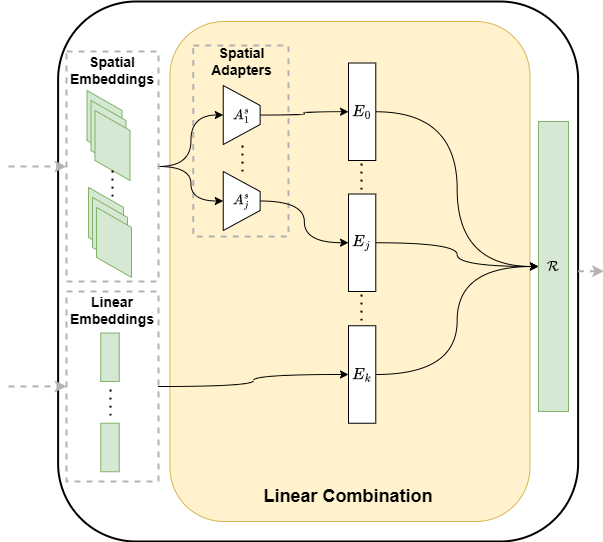
\includegraphics[width=\textwidth]{images/lin}
        \caption{\texttt{LIN}}
        \label{fig:lin}
    \end{subfigure}
    \hfill
    \begin{subfigure}[b]{0.49\textwidth}
        \centering
        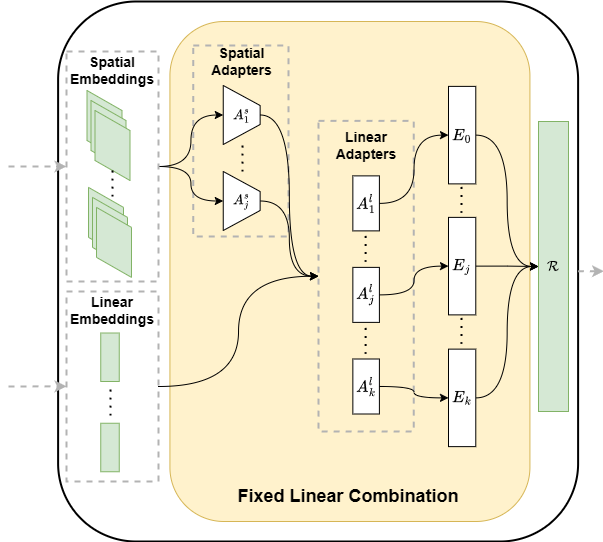
\includegraphics[width=\textwidth]{images/fix}
        \caption{\texttt{FIX}}
        \label{fig:fix_lin}
    \end{subfigure}

    \caption{In Figure we show the architecture of the Linear Combination Module (LIN) and the Fixed Linear Combination Module (FIX). In LIN, the embeddings of each model are first flattened to one-dimensional vectors, then concatenated to create a large feature vector. In FIX, the embeddings are also mapped into an embedding of fixed dimensions using $k$ different linear layers with the same size and then concatenated}
    \label{fig:lin_combination}
\end{figure}




\subsubsection{Convolutional Combination Modules}
\label{subsubsec:convolutional_combination}
In this combination module, we exploit the fact that FMs operate in the spatial field.
In fact, flatting the feature maps and concatenating them as in the linear combination modules may not be the best choice, as the spatial information is lost.
To overcome this issue, after applying the usual preprocessing step consisting of the spatial adapters, we reshaped the one-dimensional embeddings into spatial ones, to match the dimensions of the other representations.
Then, the embeddings are \textbf{concatenated along the channel dimension} and passed to one or more convolutional layers $\mathcal{A}^c$ to extract features.
At this point, the output of the convolutional layer is flattened to constitute the final representation $\mathcal{R}$, and the embedding is passed to the rest of the network.
We refer to this combination module as \textit{CNN}.

This module is particularly useful when the FMs are designed to capture spatial information, as in the case of images, but there may be cases where the FMs are not designed to capture spatial information.
Assuming that the set of FMs is composed of models that operate in the spatial field and models that operate in the linear one, we can exploit these two types of models to create a more complex combination module.
As before, first we preprocess the output of the FMs using the spatial adapters.
Then, we concatenate the FMs embedding that operate in the spatial field along the channel dimension.
We then pass this embedding through a convolutional layer to extract spatial features, followed by a ReLU activation function.
Finally, we flatten the output of the convolutional layer and concatenate it with the embeddings of the linear FMs to create the final representation $\mathcal{R}$.
We call this combination module \textit{MIX} as it is a mixture of the previous two modules.

Figure~\ref{fig:conv_combination} shows the architecture of the two convolutional combination modules.

\begin{figure}[ht]
    \centering
    \begin{subfigure}[b]{0.49\textwidth}
        \centering
        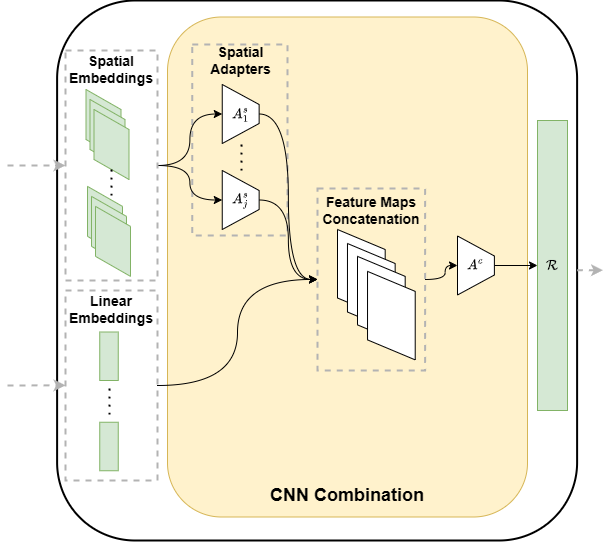
\includegraphics[width=\textwidth]{images/cnn}
        \caption{\texttt{CNN}}
        \label{fig:cnn}
    \end{subfigure}
    \hfill
    \begin{subfigure}[b]{0.49\textwidth}
        \centering
        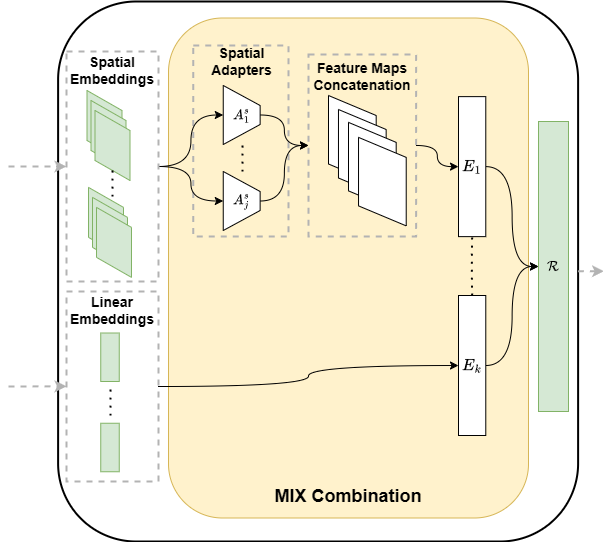
\includegraphics[width=\textwidth]{images/mix}
        \caption{\texttt{MIX}}
        \label{fig:mix}
    \end{subfigure}

    \caption{n Figure we show the architecture of the Convolutional Combination Module (CNN) and the Mixed Combination Module (MIX). In CNN, we first reshape all embedding such that can be concatened along the channel dimension. Then we use a CNN to extract feature and produce the representation $\mathcal{R}$. In MIX, first we concatenate the spatial embeddings together, then we flatten their representaion to a linear one and concatenate all the linear embeddings.}
    \label{fig:conv_combination}
\end{figure}

\subsubsection{Reservoir Combination Module}
\label{subsubsec:reservoir_combination}
Inspired by the work of \citet{gallicchio2017}, we decided to explore reservoir dynamics properties to map the input into a lower-dimension latent space using a non-linear transformation.
To develop this combination module, we created a reservoir with fixed weights using a predefined number of neurons.
As input, for the reservoir we used the representation $\mathcal{R}$ built by the LIN combination module.
The output of the reservoir is a vector of the size of the number of neurons on it.
This is the new computed representation $\mathcal{R}$, which is used as input to the policy learning network.
We refer to this combination module as \textit{RES}.
Figure~\ref{fig:reservoir_combination} shows the architecture of the reservoir combination module.

\subsubsection{DotProduct Attention Combination Module}
\label{subsubsec:dpa}

We also explored the possibility of combining representations using different types of attention-like mechanisms conditioned on the configuration of the environment.
In this case, we used the \textit{scaled dot product attention}~\citep{vaswani2017attention}.
As for the WSA module, the pre-trained model representations are reduced to a vector of fixed size using the spatial and linear adapters.
These are then stacked together to form a tensor of shape $(k \times \text{vector\_size})$, where $k$ are the number of available FMs, and $vector\_size$ is the fixed dimension of each pre-trained model embedding.
This constitutes the \textbf{key} part and the \textbf{value} part of the attention module.
For the \textbf{query} part, we used the same procedure as for the WSA module to produce the context $\mathcal{C}$.
We used the State Encoder to encode the current state of the game in a latent space, and we used an adapter to obtain a vector of the same dimensions.
As the name of the module suggests, the attention module first computes the dot product of the query with the keys, divided by the square root of the dimension of the query, then it uses a softmax function to obtain the weights.
Finally, the output of the module is computed as the dot product of the weights with the values.
We call this combination module \textit{DPA} and in Fig.~\ref{fig:dpa_combination} we show the architecture of the module.


\begin{figure}[ht]
    \centering
    \begin{subfigure}[b]{0.49\textwidth}
        \centering
        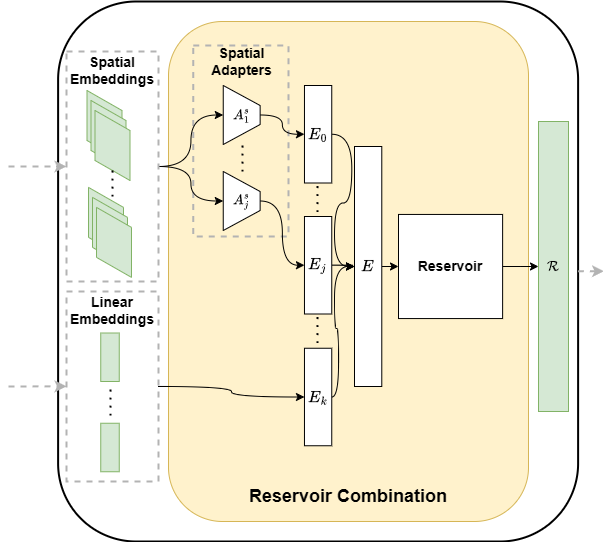
\includegraphics[width=\textwidth]{images/res}
        \caption{\texttt{RES}}
        \label{fig:reservoir_combination}
    \end{subfigure}
    \hfill
    \begin{subfigure}[b]{0.49\textwidth}
        \centering
        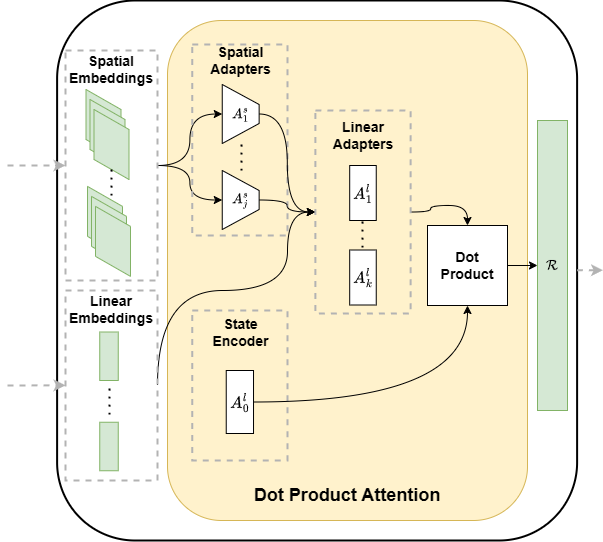
\includegraphics[width=\textwidth]{images/dpa}
        \caption{\texttt{DPA}}
        \label{fig:dpa}
    \end{subfigure}

    \caption{n Figure we show the architecture of the Reservoir Combination Module (RES) and the DotProduct Attention Combination Module (DPA). In RES, we use reservoir dynamics to encode information coming from different FMs. In DPA, the embeddings are mapped into an embedding of fixed dimensions using $k$ different linear layers with the same size and we use the State Encoder $\varepsilon$ as context $\mathcal{C}$, as for WSA.}
    \label{fig:dpa_combination}
\end{figure}



\section{Policy Learning}\label{sec:policy_learning}
This is the last part of the agent's architecture, where the enriched representation obtained from the Feature Extractor module is used to map the current state to an action.
It receives as input the enriched representation $\mathcal{R}$ as a one-dimensional vector.
$\mathcal{R}$ is assumed to contain all the relevant information, simplifying the learning process of the agent.
The Policy Learning network is a small fully-connected neural network that takes as input t$\mathcal{R}$ and outputs the probability distribution over the possible actions or the value function.
The network generally is composed of just one layer with a small number of neurons.
Eventually, the size of this network can be increased to improve the performance of the agent by increasing the number of layers and adding non-linearity.